\section{Agent-Based Simulations}
\label{sec:section4}  
\subsection{Steady-State Convergence}
Given the lack of accessible SBDP user data, I developed on agent-based simulation environment to explore the evolution of both behavioural and market-level dynamics under the above theoretical foundation. 
Agent-based modelling (ABM) is used to study how \textit{``macro phenomena emerges from micro level behaviour among a heterogeneous set of interacting agents''} \citep{janssen2005agent}, and it has been successfully applied by recent work on matching platforms \citep{immorlica2021designing} to help identify and understand the structure of equilibria, which can be computationally expensive to approximate (and in some cases even non-existent).

\begin{figure}[ht]
    \centering
    \caption{Agent-Based Simulation Convergence}
    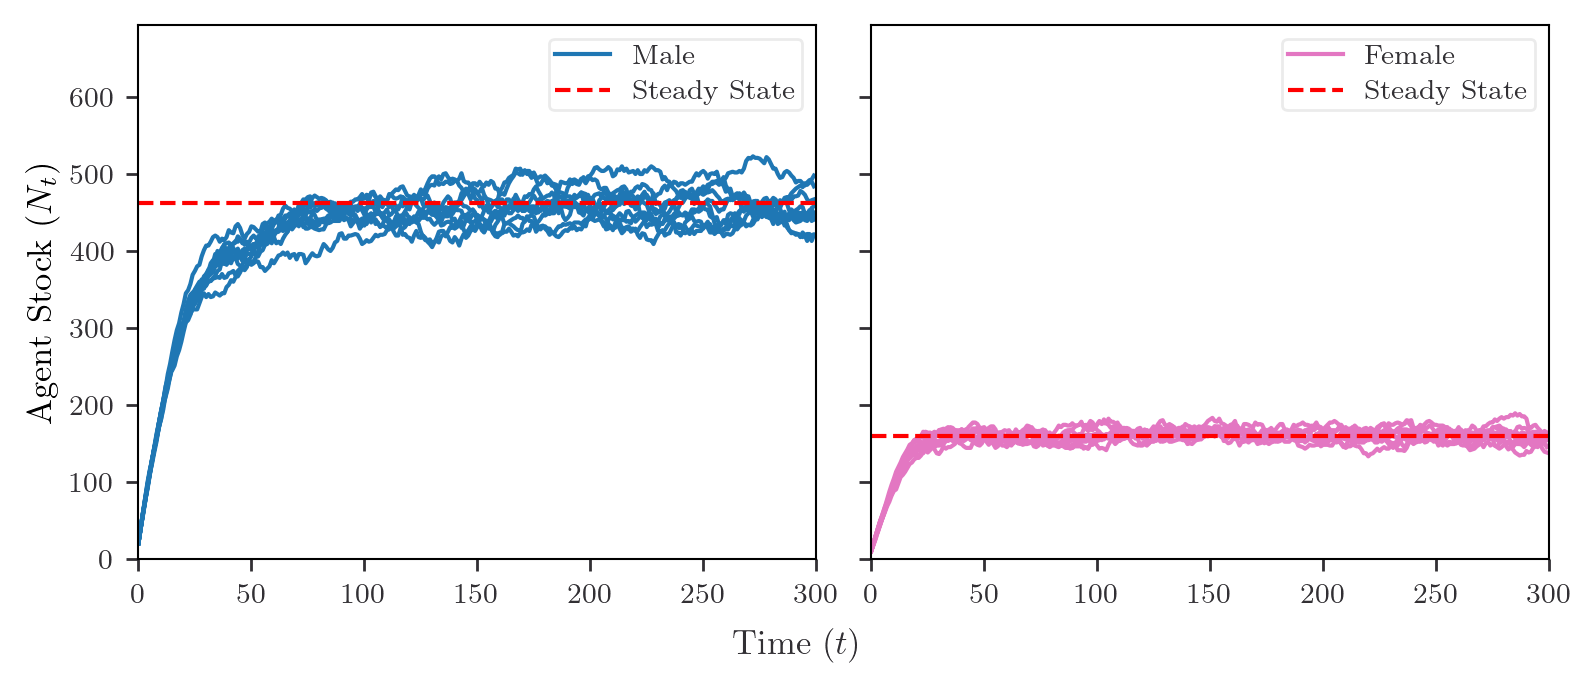
\includegraphics{abm-conv-imbalanced.png}
    \label{fig:abm-conv} 
\end{figure}

To start, I explore the convergence and stability of the SBDP market under arbitrary exogenous settings. 
In particular, \autoref{fig:abm-conv} shows the evolution of (sex-specific) agent masses for 10 independent simulation batches, over 300 time periods, and with a 2:1 ratio between male and female arrival flows. 
These simulations were conducted under partially rational expectation conditions; that is, with agents using optimal policies for some fixed steady-state even when this is not actually the current platform state.  
As evident from these results, this process converges onto the SE computed using the procedures in \autoref{sec:section3.1}. 
Furthermore, the ABM simulations show that the long side of the market (males) takes considerably longer to converge onto its steady-state level. 
One technical point worth noting is that the above simulations involve a finite number of agents as opposed to \textit{agent masses}, as per our continuum model.  
Nevertheless, I examine the limiting case of these dynamics, with \autoref{fig:abm-conv-ssize} depicting how, by the law of large numbers, stationary deviations around the steady-state level become negligible as the number of agents in the platform tends to infinity. 

\begin{figure}[ht] 
    \centering
    \caption{Agent-Based Simulation Convergence with Varying Sample Sizes}
    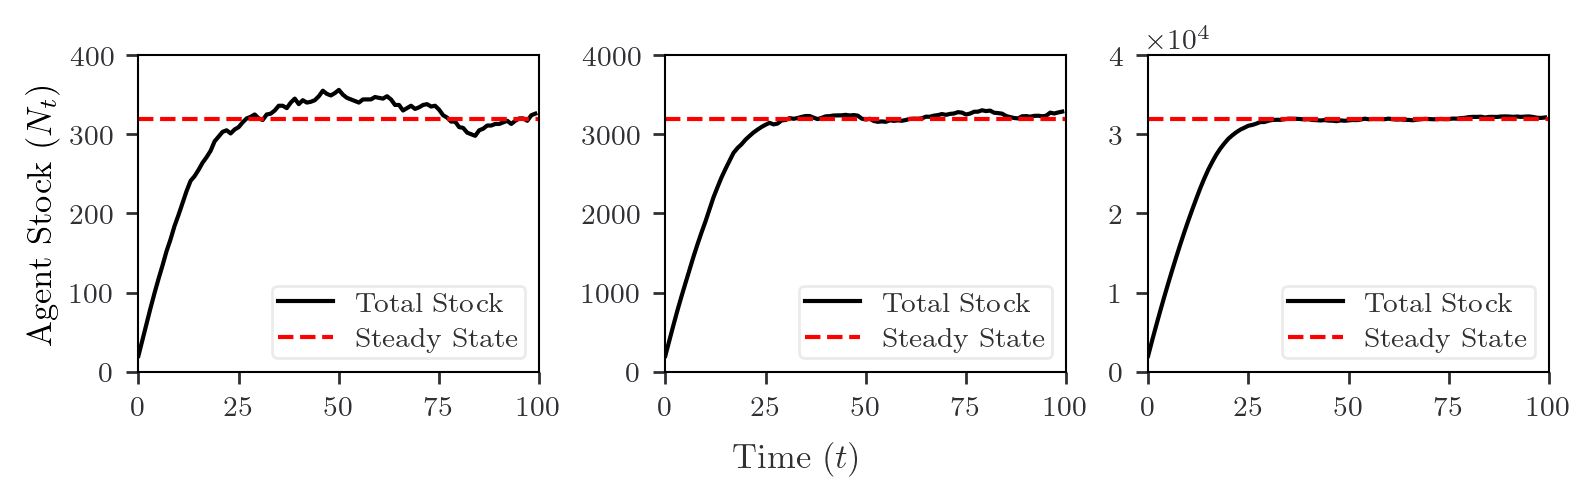
\includegraphics{abm-conv-ssize.png}
    \label{fig:abm-conv-ssize}
\end{figure} 

\subsection{Myopic Best-Response Dynamics}
Finally, I simulate the SBDP market under myopic best-response dynamics \citep{fudenberg1998theory} to explore whether if SE can be attained using a more robust process of gameplay. 
For this simulation, agents re-compute their optimal policies at the start of every time period given the current market state, unlike in the previous scenario where optimal policies are computed once with respect to the SE for some given exogenous settings. 
This process is \textit{myopic} in the sense that agent policies account only for the current platform state but not for its dynamic evolution; yet it is still more robust than the previous experiment as echoing feedback between policy and state updates could create outward-spiralling dynamics that prevent convergence onto SE. 
The results of these simulations over 120 time periods are presented in \autoref{fig:abm-br}, showing that, both in the case of balanced and unbalanced markets, the SE can be attained using myopic best response dynamics.

\begin{figure}[ht] 
    \centering
    \caption{Agent-Based Simulation Under Myopic Best Response Dynamics}
    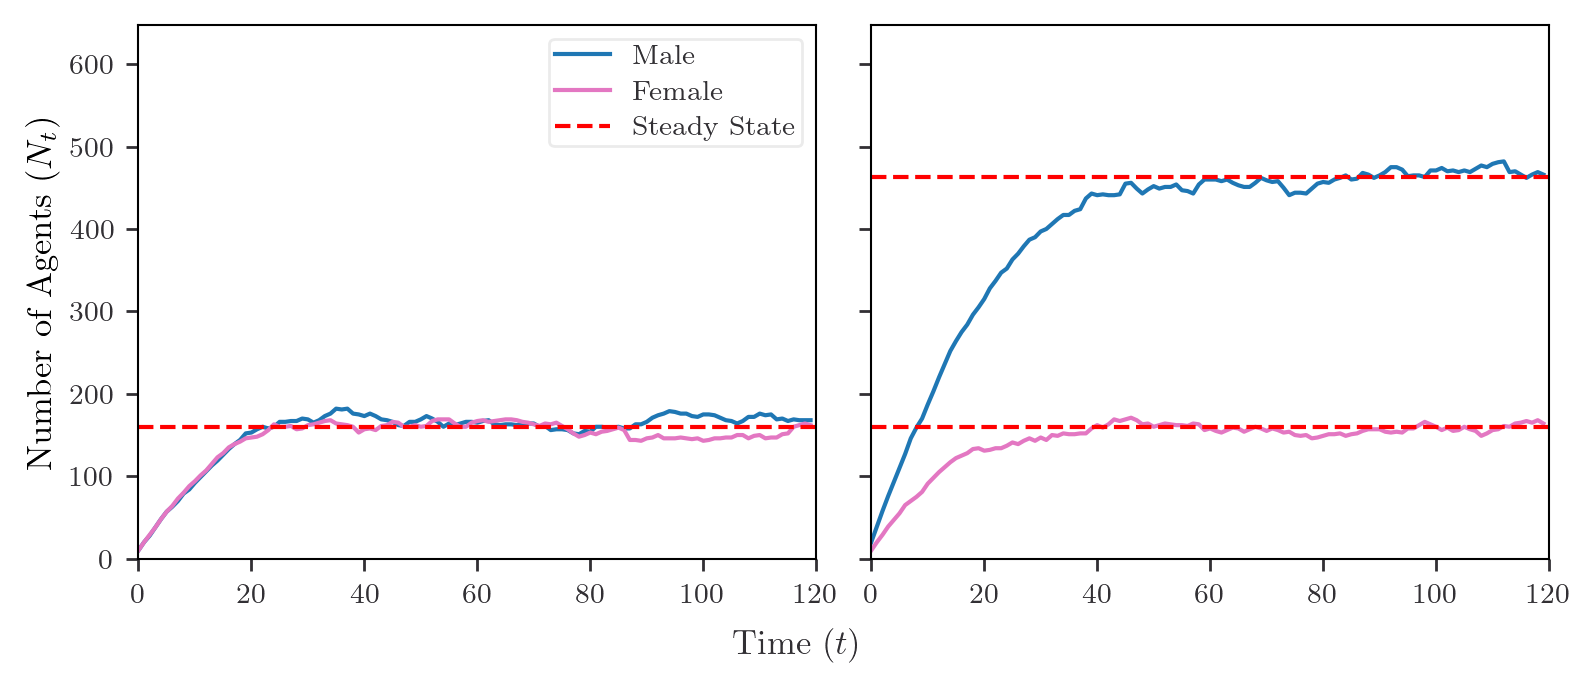
\includegraphics{abm-br.png}
    \label{fig:abm-br}
\end{figure}   